\documentclass[a4paper]{article} %format de la feuille + type de document https://en.wikibooks.org/wiki/LaTeX/Document_Structure#Document_classes
%packages nécessaire pour nos besoins
\usepackage[utf8]{inputenc}
\usepackage[T1]{fontenc}
\usepackage[english,french]{babel}
\usepackage{amsmath}
\usepackage{amssymb,amsfonts,textcomp}
\usepackage{color}
\usepackage{array}
\usepackage{supertabular}
\usepackage{hhline}
\usepackage{hyperref}
\usepackage{capt-of}
\usepackage[pdftex]{graphicx}
\usepackage{sectsty}
\usepackage{tcolorbox}
\usepackage{textcomp}
\usepackage{courier}
\usepackage[font={small,it}]{caption}
\usepackage{float}
\usepackage{graphicx}
\usepackage{subcaption}
\usepackage{caption}


%Définition des couleurs
\definecolor{havelockBlue}{rgb}{0.004, 0.42, 0.73}
\definecolor{Monokaimagenta}{rgb}{0.86,0.08,0.24}

%utilisation de la couleur définie avant
%toutes les sections auront cette couleur
\sectionfont{\color{havelockBlue}}
\subsectionfont{\color{havelockBlue}}
%début du document
\begin{document}

%début d'un titre
\begin{titlepage}
            %centre les éléments
	\centering
	
	{\scshape\LARGE \color{Monokaimagenta} Laboratoire \\ Universal Asynchronous Receiver Transmitter \par}
	
	%espace vertical de 1 mms
	\vspace{1cm}
	
	{\Large\itshape Johanna Melly \& Sven Rouvinez\par}
	
	%http://www.personal.ceu.hu/tex/spacebox.htm
	\vfill
	Professeur\par
	%met le texte en gras 
	\textbf{Carlos Andrés Pena} \par% ajoute une ligne 
	\vspace{1cm}
	Assistant\par
	\textbf{Gaëtan Matthey}
	
	\vfill

            %affiche la date actuelle
	{\large \today\par}
	
%fin de la page de titre
\end{titlepage}

%démarre un chapitre, les nombres se mettent automatiquement et seront incrémenté quand un autre \section est rencontré
%voir https://en.wikibooks.org/wiki/LaTeX/Document_Structure#Sectioning_commands
\section{Description générale}
On appelle « trame » une suite de bits envoyés en série. Cette trame comprend dans l’ordre :
\begin{itemize}
\item Le « start-bit » toujours égal à 0.
\item Les bits de donnée (sur n bits) à transmettre.
\item Le bit de parité facultatif (non demandé dans ce labo).
\item Le bit de stop égal à 1.
\end{itemize}
De plus, l’état de repos de la ligne est fixé à 1.
\\ 
\begin{figure}[H]
    \centering
    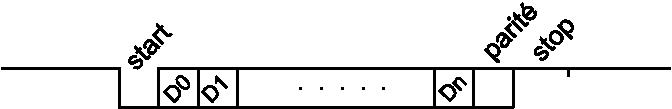
\includegraphics[width=.8\textwidth]{src/uart_1.jpg}
    \captionof{figure}{trame}
    \label{fig:trame}
\end{figure}


%saut à la ligne


%début d'un encadré avec la couleur définie plus haut
\begin{tcolorbox}[colframe=Monokaimagenta,colback=white]
Nous réalisons la partie récepteur. Le circuit se compose d'un shift register, d'un compteur, un registre de sortie et un machine à états pour le contrôle.\\
Le début de la communication démarre lorsque que le contrôle reçoit un $0$.

\begin{itemize}
    \item    Après un reset, le registre de sortie contient la valeur $0$
    \item    Détection du front descendant sur l'entrée série provoqué par le \textbf{start bit} de l'émetteur
        \begin{itemize}
            \item    \begin{figure}[H]
                        \centering
                        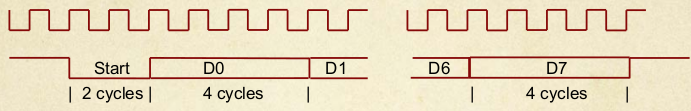
\includegraphics[width=.8\textwidth]{src/chrono_emetteur.jpg}
                        \captionof{figure}{Chronogramme émetteur}
                     \label{fig:trame}
                \end{figure}
        \end{itemize}
    \item    Chargement des bits tous les 4 cycles d'horloge après le front descendant du \textbf{start bit}
    \item    Quand la tranmission est finie, la trame est chargée dans le registre de sortie
    
\end{itemize}   
%fin de l'encadré
\end{tcolorbox}

\section{Architecture}\

\begin{tcolorbox}[colframe=Monokaimagenta,colback=white]
\paragraph{Architecture - Max 1/2 page}
Dessinez le schéma bloc complet de votre circuit. Ce circuit contient entre autre : shift-register, compteurs et machine d’état, avec les bus de données et les signaux de contrôle. Vous pouvez faire ce schéma bloc à la main (très proprement), ou en utilisant Logisim (mais avec le nom des signaux), ou avec un outil de dessin de votre choix.

Remplacez le texte ci-dessus par vos réponses (à l’intérieur du cadre rouge)\\


\end{tcolorbox}


\section {Réalisation}
\subsection{Le bloc shift-register}
Ce bloc sur 8 bits a 4 modes de fonctionnement. Vous devez le refaire entièrement avec des bascules et des multiplexeurs.
\begin{tcolorbox}[colframe=Monokaimagenta,colback=white]
\paragraph{Conception et tests - Max 1 page}
Insérez une capture d’écran pour présenter votre bloc shift-register. Expliquez brièvement son fonctionnement.
Indiquez comment vous avez testé les 4 modes de fonctionnement afin de le valider.
Remplacez le texte ci-dessus par vos réponses (à l’intérieur du cadre rouge)
\\
\end{tcolorbox}
\subsection{Le bloc compteur 0-3}
Le premier compteur demandé compte de 0 à 3. Ce compteur comprend une entrée de remise à 0 synchrone et une sortie indiquant que le compteur a atteint sa valeur maximum.
\begin{tcolorbox}[colframe=Monokaimagenta,colback=white]
\paragraph{Conception et tests - Max 1 page }
\begin{figure}[H]
\centering
    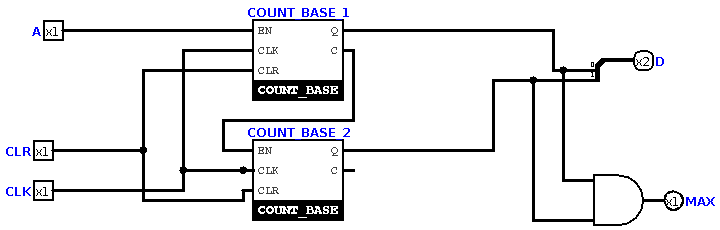
\includegraphics[width=.8\textwidth]{src/COUNT_4BITS.png}
    \captionof{figure}{Compteur 0\-3}
    \label{fig:count4bits}
\end{figure}
Insérez une capture d’écran pour présenter votre bloc compteur 0-3. Expliquez sa réalisation et son fonctionnement.
Indiquez comment vous avez testé les différents modes de fonctionnement afin de le valider. Vous pouvez ajouter un chronogramme.
Remplacez le texte ci-dessus par vos réponses (à l’intérieur du cadre rouge)


Ce bloc est composé d'un bloc de base (voir \ref{fig:countBase}) qui s'occupe uniqument de changer d'étât une bascule D, ce qui aura comme effet de compter lorsque qu'il est connecté avec d'autres de ces blocs.\\
\paragraph{Définition des entrées}
\begin{itemize}

    \item     \textbf{A} active le compteur
    \item     \textbf{CLK} permet de connecter l'horloge du circuit "maître"
    \item     \textbf{CLR} permet une remise à zéro du compteur

\end{itemize}

\paragraph{Définition des sorties}
\begin{itemize}

    \item     \textbf{MAX} s'active lorsque que le compteur à atteint sa valeur maximum, c'est-à-dire 3.
    \item     \textbf{D} affiche l'état du compteur
\end{itemize}


\end{tcolorbox}
\subsection{Le bloc compteur 0-7}
Le deuxième compteur demandé compte de 0 à 7. Ce compteur comprend une entrée de remise à 0 synchrone, une entrée enable pour l’activer et une sortie indiquant que le compteur a atteint sa valeur maximum.
\begin{tcolorbox}[colframe=Monokaimagenta,colback=white]
\paragraph{Conception et tests - Max 1 page}
Insérez une capture d’écran pour présenter votre bloc compteur 0-7. Expliquez sa réalisation et son fonctionnement. Inutile de reprendre les explications du paragraphe précédent 3.2. Expliquez simplement ce que vous avez dû changer ou rajouter pour passer du compteur 0-3 au compteur 0-7.
Indiquez comment vous avez testé les différents modes de fonctionnement afin de le valider. Vous pouvez ajouter un chronogramme.
Remplacez le texte ci-dessus par vos réponses (à l’intérieur du cadre rouge)
\\
\end{tcolorbox}
\subsection{La machine d’état}
Cette machine d’état de type 1 parmi M contrôle les deux compteurs et le shift register. 
\begin{tcolorbox}[colframe=Monokaimagenta,colback=white]
\paragraph{Conception Max 3 pages}
Précisez les entrées et sorties de votre machine d’état
Cette machine d'état prend en entrée le compteur 4 bits, le compteur 8 bits et le bit envoyé par l'émetteur. Les bascules bistables sont de type S-R car il fallait qu'elle ne change pas d'état après être passée à 1 au flanc montant. Cette machine d'état va renvoyer un 1 si un '0' à été transmis comme signal de départ et si 8 coups d'horloges n'ont pas encore été atteints.
La première bascule prend en entrée l'inverse du bit envoyé par l'émetteur (de façon à ce que l'horloge passe à 1 lorsuqe le bit envoyé ets un 0) et, en horloge, le compteur 4 bits (puisque les bits de l'émetteur doivent être reçus chaque 4 coups d'horloge). Ainsi, à chaque 4 coups d'horloge, l'horloge de la première bascule va passer à 1, et si l'entrée de S de la bascule est à 1 (et donc le bit envoyé par l'émetteur à 0), l'état de la bascule va passer à 1 et y rester. Ainsi, on sait que le bit qui signale le départ à été envoyé.
La deuxième bascule prend en entrée le compteur 8 bits, et en horloge le compteur 4 bits. Ainsi, chaque 4 coups d'horloge, la bascule va "contrôler" que l'on n'ait pas atteint la fin du mot. Si l'entrée est à 1 lorsque le compteur 8 bit annonce la fin du mot, la bascule change d'état et y reste.
Au bout du circuit, une porte XOR permet de savoir si les deux bascules ne sont pas au même état.
Ainsi, au départ, la sortie est à 0. Dès qu'un 0 est transmis par l'émetteur, la première bascule passe à 1, et la sortie sera à 1 également. Puis, dès qu'on atteint les 8 coups de clock, la deuxième bascule passe à 1 aussi, et la sortie passe donc définitivement à 0.

Insérez un graphe des états et une table des états. Donnez des explications sur le fonctionnement de votre machine. Quel est son Type ?
Donnez les équations des états futurs et insérez une capture d’écran de la réalisation de votre machine.
Remplacez le texte ci-dessus par vos réponses (à l’intérieur du cadre rouge)
\\
\end{tcolorbox}
\section {Intégration et simulation}
\subsection{Intégration}
Suivant votre partie à concevoir, vous devez réaliser l’UART en interconnectant les différents blocs. 
\begin{tcolorbox}[colframe=Monokaimagenta,colback=white]
\paragraph{Réalisation et simulation Logisim - Max 1 page}
Insérez une capture d’écran de l’UART complet sous Logisim
Expliquez le fonctionnement global de l’UART
Remplacez le texte ci-dessus par vos réponses (à l’intérieur du cadre rouge)
\\
\end{tcolorbox}
 \subsection{Simulation sous Logisim}
L’UART réalisé est ensuite testé en simulation sous Logisim.
\begin{tcolorbox}[colframe=Monokaimagenta,colback=white]
\paragraph{Réalisation et simulation Logisim - Max 2 pages}
Indiquez comment vous simulez votre UART sous Logisim (seul ou avec le générateur fourni), ET avec un UART d’un autre groupe (indiquez quel groupe)
Insérez un ou plusieurs chronogrammes, annotez-le(s) et expliquez pourquoi le fonctionnement est correct et conforme aux spécifications.
Remplacez le texte ci-dessus par vos réponses (à l’intérieur du cadre rouge)
\\
\end{tcolorbox}
 \subsection{Synthèse et test de fonctionnement réel}
Synthèse et configuration du matériel, test de fonctionnement.
L’UART finalement synthétisé et chargé dans une carte, une carte émetteur sera reliée à une carte récepteur afin de tester une transmission de données.
\begin{tcolorbox}[colframe=Monokaimagenta,colback=white]
\paragraph{Essais avec une carte - Max 1 page}
Indiquez comment vous faites le test (et avec un groupe différent de la simulation). Quelles données choisissez-vous pour faire les essais ?Vous devez faire valider votre circuit en fonctionnement au professeur ou à l’assistant
Commentez brièvement votre expérience dans cette étape en mentionnant, par exemple, des éventuelles difficultés à faire fonctionner le circuit ou à configurer la carte, etc.
Remplacez le texte ci-dessus par vos réponses (à l’intérieur du cadre rouge)
\\
\end{tcolorbox}
\section {Conclusion}
\begin{tcolorbox}[colframe=Monokaimagenta,colback=white]
\paragraph{Conclusion - Max 1/2 page}
Cette section est libre pour que vous fassiez une analyse critique de votre laboratoire
Commentez et analysez 
les résultats, 
les difficultés et les succès
Rédigez quelques conclusions personnelles
Donnez vos impressions et analysez votre expérience dans ce laboratoire
Discutez de ce que vous avez appris (ou pas)
Analysez votre travail, votre implication
Evitez les banalités et les lieux communs
ETCAETERA…
\\
\end{tcolorbox}

\section{Annexe}


\begin{figure}[H]
\centering
    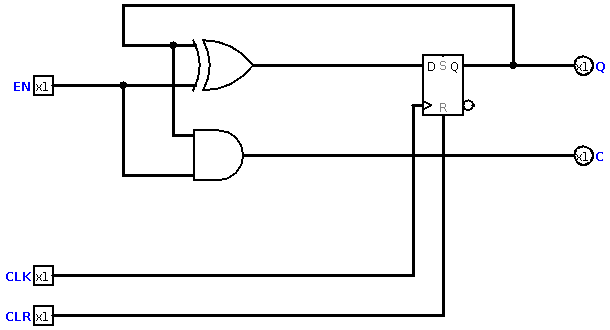
\includegraphics[width=.8\textwidth]{src/COUNT_BASE.png}
    \captionof{figure}{Circuit de base des compteurs}
    \label{fig:countBase}
    \end{figure}


\end{document}